\documentclass{standalone}

\usepackage[latin1]{inputenc}
\usepackage{tikz}

\usetikzlibrary{calc}
\usetikzlibrary{arrows.meta}

\begin{document}

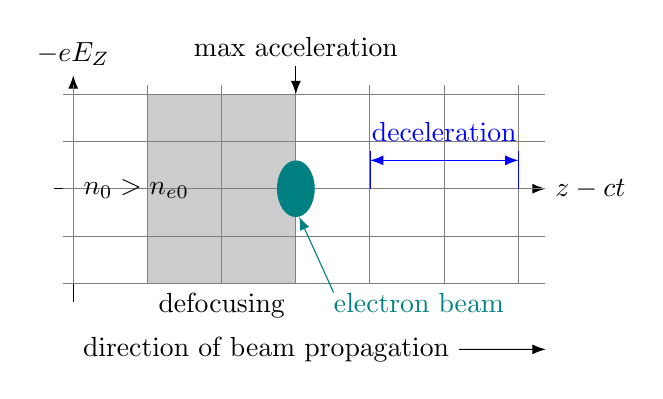
\begin{tikzpicture}[scale=1.2,domain=0:5]

	% defocusing rectangle
	\fill[black!40!white, opacity=0.5] (pi/4,1) rectangle (3*pi/4,-1);
	\draw (pi/2,-1) node[color=black,anchor=north] {defocusing};

	% axis and grid
	\draw[-Latex] (-0.2,0) -- (5,0) node[right] {$z-ct$};
	\draw[-Latex] (0,-1.2) -- (0,1.2) node[above] {$-eE_Z$};
	\draw[very thin,color=gray,xshift=-0.1,xstep=pi/4,ystep=0.5] (-0.1,-1) grid (5,1.1);

	% sin curve
	\draw[color=red,smooth,thick,samples=200] plot[id=-sin] function{-sin(2*x)}
	node[color=black,right] {$n_0>n_{e0}$};

	% deceleration
	\draw[blue] (pi,0) -- (pi,0.4);
	\draw[blue] (3*pi/2,0) -- (3*pi/2,0.4);
	\draw[blue,Latex-Latex] (pi,0.3) -- node {} (3*pi/2,0.3);
	\draw[blue] (5*pi/4,0.4) node[anchor=south] {deceleration};

	%electron bunch
	\fill[blue!50!green] (3*pi/4,0) ellipse (0.2 and 0.3);
	\draw[blue!50!green] (3*pi/4+0.3,-1) node[anchor=north west] {electron beam};
	\draw[blue!50!green,-Latex] (3*pi/4+0.4,-1.1) -- ($(3*pi/4,0)+(-80:0.2 and 0.3)$);

	% max acc
	\draw[-Latex] (3*pi/4,1.3) node[anchor=south] {max acceleration} -> (3*pi/4,1);

	\draw (0,-1.7) node[anchor=west](dir) {direction of beam propagation};
	\draw[-Latex] (dir.east) -> (5,-1.7);
\end{tikzpicture}


\end{document}
